\chapter{The projective plane}\label{chapter:projective.plane}%
\section{The projective line}
A cubic polynomial in one variable might have three roots:
\begin{center}
\documentclass[tikz]{standalone}
\usepackage{pgfplots}
\colorlet{curveZero}{gray!75}
\colorlet{curveOne}{blue!60}
\colorlet{curveTwo}{brown!50!gray}
\colorlet{curveThree}{green!40!gray}
\colorlet{curveFour}{red!50!gray}
\NewDocumentCommand\DrawDotInPlot{O{}mmO{}}%
{%
\fill[gray!20,draw=gray] (axis cs:{#2},{#3}) circle (1.3pt) node[above,black,#4] {\(#1\)};%
}%
\NewDocumentCommand\DrawDot{O{}mmO{}}%
{%
\fill[gray!20,draw=gray] ({#2},{#3}) circle (1.3pt) node[above,black,#4] {\(#1\)};%
}%
\NewDocumentCommand\DrawNode{O{}m}%
{%
\fill[gray!20,draw=gray] (#2) circle (1.3pt) node[above,black] {\(#1\)};%
}%
\colorlet{axisColor}{gray!50}
\tikzstyle{shapeZero}=[fill=curveZero,opacity=.4]
\tikzstyle{shapeOne}=[fill=curveOne,opacity=.4]
\tikzstyle{shapeTwo}=[fill=curveTwo,opacity=.4]
\tikzstyle{shapeThree}=[fill=curveThree,opacity=.4]
\tikzstyle{groupElementLabel}=[minimum size=2.4em]
\tikzstyle{groupElement}=[minimum size=2.4em,shapeZero,draw=curveZero]
\tikzstyle{cosetOne}=[minimum size=2.4em,shapeOne,draw=curveOne]
\tikzstyle{cosetTwo}=[minimum size=2.4em,shapeTwo,draw=curveTwo]


\begin{document}
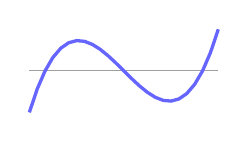
\begin{tikzpicture}
\draw[curveZero] (-1.2,0) -- (1.2,0);
\draw[very thick,curveOne,domain=-1.2:1.2] plot (\x,{\x*(\x-1)*(\x+1)});
%\draw[very thick,curveTwo,domain=-1:1] plot (\x,{-.5*\x*\x*\x});
\DrawDot{0}{0}
\DrawDot{-1}{0}
\DrawDot{1}{0}
%\fill[curveOne] (0,0) circle (2pt);
%\fill[curveOne] (-1,0) circle (2pt);
%\fill[curveOne] (1,0) circle (2pt);
%\draw[very thick,curveThree,domain=-1:1] plot (\x,{-1+.25*\x*\x*\x});
\end{tikzpicture}
\end{document}
\end{center}
We can put them wherever we like by picking suitable coefficients.
Imagine one of them moves far away, so at time \(t\), we want our roots to be at \(x=0,x=1,x=t\).
We could pick the polynomial to be \(x(x-1)(x-t)\); but this has no limit as \(t\) gets large, 
since there is a factor of \(t\) in our polynomial.
Fix this: divide out by \(t\), say take our polynomial to be instead \(x(x-1)(x-t)/t\), which does not change the roots.
Expand this out:
\[
\frac{x(x-1)(x-t)}{t}=\frac{x^3}{t}-\left(1+\frac{1}{t}\right)x^2+x.
\]
For nonzero \(t\), the coefficients remain bounded as \(t\) gets large.
\begin{center}
\input{tikz-3-roots-move}
\end{center}
So our root moves far away, while the coefficients remain bounded.
What happens as \(t\) becomes infinite?
\begin{center}
\documentclass[tikz]{standalone}
\usepackage{pgfplots}
\colorlet{curveZero}{gray!75}
\colorlet{curveOne}{blue!60}
\colorlet{curveTwo}{brown!50!gray}
\colorlet{curveThree}{green!40!gray}
\colorlet{curveFour}{red!50!gray}
\NewDocumentCommand\DrawDotInPlot{O{}mmO{}}%
{%
\fill[gray!20,draw=gray] (axis cs:{#2},{#3}) circle (1.3pt) node[above,black,#4] {\(#1\)};%
}%
\NewDocumentCommand\DrawDot{O{}mmO{}}%
{%
\fill[gray!20,draw=gray] ({#2},{#3}) circle (1.3pt) node[above,black,#4] {\(#1\)};%
}%
\NewDocumentCommand\DrawNode{O{}m}%
{%
\fill[gray!20,draw=gray] (#2) circle (1.3pt) node[above,black] {\(#1\)};%
}%
\colorlet{axisColor}{gray!50}
\tikzstyle{shapeZero}=[fill=curveZero,opacity=.4]
\tikzstyle{shapeOne}=[fill=curveOne,opacity=.4]
\tikzstyle{shapeTwo}=[fill=curveTwo,opacity=.4]
\tikzstyle{shapeThree}=[fill=curveThree,opacity=.4]
\tikzstyle{groupElementLabel}=[minimum size=2.4em]
\tikzstyle{groupElement}=[minimum size=2.4em,shapeZero,draw=curveZero]
\tikzstyle{cosetOne}=[minimum size=2.4em,shapeOne,draw=curveOne]
\tikzstyle{cosetTwo}=[minimum size=2.4em,shapeTwo,draw=curveTwo]


\begin{document}
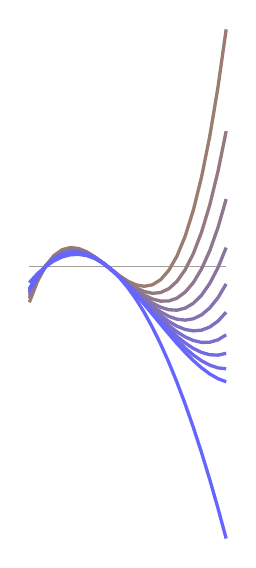
\begin{tikzpicture}
\draw[curveZero] (-1,0) -- (1.5,0);
%\draw[very thick,curveTwo,domain=-1:1] plot (\x,{-.5*\x*\x*\x});
%\fill[curveOne] (0,0) circle (2pt);
%\fill[curveOne] (-.8,0) circle (2pt);
\foreach \i/\j in {.8/10,1/20,1.2/30,1.4/40,1.6/50,1.8/60,2/70,2.2/80,2.4/90,2.6/100}
{
	\draw[very thick,curveOne!\j!curveTwo,domain=-1:1.5] plot (\x,{\x*(\x/\i-1)*(\x+.8)});
}
\draw[very thick,curveOne,domain=-1:1.5] plot (\x,{\x*(-1)*(\x+.8)});
\DrawDot{0}{0}
\DrawDot{-.8}{0}
%\fill[curveOne] (.8,0) circle (2pt);
%\draw[very thick,curveThree,domain=-1:1] plot (\x,{-1+.25*\x*\x*\x});
\end{tikzpicture}
\end{document}
\end{center}
Our polynomial reaches a limit
\[
-x^2+x=x(1-x).
\]
The two fixed roots stay in place, but the polynomial drops degree when the moving root disappears to infinity.

There is something frustrating about the possibility that a moving polynomial can drop degree like this, so that in the limit, roots can disappear to infinity.
Consider how we can ``hold on'' to the roots.
Take a cubic polynomial
\[
p(x)=ax^3+bx^2+cx+d.
\]
Associate to it the homogeneous polynomial in two variables
\[
P(x,y)=ax^3+bx^2y+cxy^2+dy^3
\]
by sticking in a power of \(y\) in each term so that the term reaches total degree \(3\) in \(x\) and \(y\) together.
The original polynomial is \(p(x)=P(x,1)\).
So geometrically, \(p(x)\) is just \(P(x,y)\) but only calculated along the line \(y=1\).
\begin{problem}{projective.plane:homog}
Homogenize \(p(x)=x^4+x+1\).
\end{problem}
\begin{answer}{projective.plane:homog}
\(P(x,y)=x^4+xy^3+y^4\)
\end{answer}
All terms have total degree \(3\) so, when we rescale the variables, every term scales by \(3\) factors of the scaling
\[
P(sx,sy)=s^3P(x,y)
\]
In particular, if \(P(x,y)\) vanishes at some point \((x,y)=(x_0,y_0)\) of the plane, it also vanishes at every rescaling of that point.
So it also vanishes on the line through \((x_0,y_0)\) and \((0,0)\).
Thus the zeroes of a homogeneous polynomial form a collection of lines through the origin.
\begin{example}
Taking \(p(x)=x(x-1)(x+1)\), we find
\[
P(x,y)=x(x-y)(x+y)
\]
by making each factor homogeneous.
On the graph of \(P(x,y)\) we see the graph of \(p(x)\) along the line \(y=1\):
\begin{center}
\documentclass{standalone}
\usepackage{pgfplots}
\pgfplotsset{width=7cm,compat=1.17}
\usepgfplotslibrary{fillbetween}
\begin{document}
\begin{tikzpicture}
\begin{axis}[
%height=15cm,
%hide axis,
%axis lines=center,
%axis on top,
%axis line style={draw=none},
%tick style={draw=none},
xtick=\empty,
ytick=\empty,
ztick=\empty,
]
\newcommand{\xxx}{1.51}
\newcommand{\rrr}{-1}
\addplot3+[name path=A,blue,domain=-\xxx:\xxx,samples=60,samples y=0,mark=none] 
		({x},
		 {-1},
		 {20*(-\xxx)*(-\xxx-\rrr)*(-\xxx-1)});
\addplot3 [
surf,
shader=flat,
%faceted color=gray,
samples=30,
domain=-\xxx:\xxx,y domain=-1:1
] {20*x*(x+y)*(x+\rrr*y)};
\addplot3+[name path=B,blue,very thick,domain=-\xxx:\xxx,samples=60,samples y=0,mark=none] 
		({x},
		 {-1},
		 {20*x*(x-\rrr)*(x-1)});
\addplot3[gray!40] fill between[of=A and B];
%\addplot3+[black,thick,domain=-1:1,samples=60,samples y=0,mark=none] 
%		({0},
%		 {x},
%		 {0});
%\addplot3+[black,thick,domain=-1:1,samples=60,samples y=0,mark=none] 
%		({-x},
%		 {x},
%		 {0});
%\addplot3+[black,thick,domain=-1:1,samples=60,samples y=0,mark=none] 
%		({-\rrr*x},
%		 {x},
%		 {0});
\end{axis}
\end{tikzpicture}
\end{document}
\end{center}
So \(P(x,y)\) vanishes on the lines \(x=0\), \(x=y\), \(x=-y\) in the plane.
These lines intersect the line \(y=1\) at \(x=0\), \(x=1\), \(x=-1\), the roots of \(p(x)\).
\begin{center}
\input{tikz-homogenizing-2}
\end{center}
\end{example}
\begin{problem}{projective.plane:homog.2}
Starting with \(p(x)=x^3+x\), compute \(P(x,y)\), find the real roots of \(p(x)\) and the lines through the origin on which \(P(x,y)\) vanishes.
Draw the graph of \(P(x,y)\); indicate on it where the graph of \(p(x)\) lies.
\end{problem}
Passing from the polynomial \(p(x)\) to the homogeneous polynomial \(P(x,y)\), we lose no information, since \(p(x)=P(x,1)\).
The same trick works for polynomials of any degree.
But the roots now behave better as we allow them to move: we picture that the lines only turn around, but they can't disappear, because they have to stay through the origin.
\begin{example}
Return to our example of 
\[
p(x)=\frac{x(x-1)(x-t)}{t}.
\]
Just think of \(t\) as a constant for now; we will soon let it move.
Homogenize:
\[
P(x,y)=\frac{x(x-y)(x-ty)}{t}.
\]
So the roots are the lines \(x=0\), \(x=y\), \(x=ty\).
As we let \(t\) get large, the line \(x=ty\) can be written as \(x/t=y\), so becomes \(0=y\) in the limit.
\end{example}
Take any polynomial \(p_t(x)\) whose coefficients depend on some parameter \(t\) (or maybe several parameters).
Imagine we compute out the associated homogeneous polynomial, call it \(P_t(x,y)\).
Suppose that \(p_t(x)\) has some degree \(d\), except maybe for certain ``special'' values of \(t\).
As long as the coefficients of \(p_t(x)\) don't all disappear at once, i.e. for the same value of \(t\) or limit of \(t\), the same is true of \(P_t(x,y)\), since they are the same coefficients.
All terms in the homogeneous polynomial \(P_t(x,y)\) have degree exactly \(d\).
Since they never all vanish, \(P_t(x,y)\) doesn't drop degree for any value or limit of \(t\).

Each point \(x\) becomes a unique point \((x,y)=(x,1)\) on the line \(y=1\).
\begin{center}
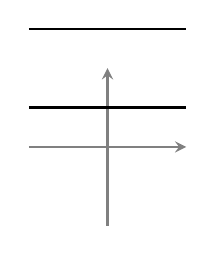
\begin{tikzpicture}
\draw[black,thick] (-1,1.5) -- (1,1.5);
\DrawDot{-.6}{1.5}
%\fill[black] (-1.2,3) circle (3pt);
\draw[gray,thick,-stealth] (-1,0) -- (1,0);
\draw[gray,thick,-stealth] (0,-1) -- (0,1);
\draw[black,thick] (-1,.5) -- (1,.5);
\DrawDot{-.6}{.5}
%\fill[black] (-1.2,1) circle (3pt);
\end{tikzpicture}
\end{center}
Conversely, each point \((x,y)=(x,1)\) arises in this way from a point \(x\).
But each point \((x,1)\) also spans a line through the origin.
\begin{center}
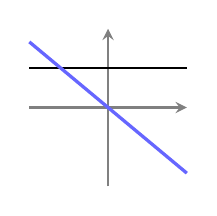
\begin{tikzpicture}
\draw[gray,thick,-stealth] (-1,0) -- (1,0);
\draw[gray,thick,-stealth] (0,-1) -- (0,1);
\draw[black,thick] (-1,.5) -- (1,.5);
\draw[curveOne,very thick] (-1,{5/6}) -- (1,{-5/6});
\DrawDot{-.6}{.5}
%\fill[black] (-1.2,1) circle (3pt);
\DrawDot{0}{0}
%\fill[curveOne] (0,0) circle (3pt);
\end{tikzpicture}
\end{center}
Every line through the origin arises uniquely in this way except \(y=0\), which we can think of as \(x=\infty\).
Spin the line around the origin.
\begin{center}
\documentclass[tikz]{standalone}
\colorlet{curveZero}{gray!75}
\colorlet{curveOne}{blue!60}
\colorlet{curveTwo}{brown!50!gray}
\colorlet{curveThree}{green!40!gray}
\colorlet{curveFour}{red!50!gray}
\NewDocumentCommand\DrawDotInPlot{O{}mmO{}}%
{%
\fill[gray!20,draw=gray] (axis cs:{#2},{#3}) circle (1.3pt) node[above,black,#4] {\(#1\)};%
}%
\NewDocumentCommand\DrawDot{O{}mmO{}}%
{%
\fill[gray!20,draw=gray] ({#2},{#3}) circle (1.3pt) node[above,black,#4] {\(#1\)};%
}%
\NewDocumentCommand\DrawNode{O{}m}%
{%
\fill[gray!20,draw=gray] (#2) circle (1.3pt) node[above,black] {\(#1\)};%
}%
\colorlet{axisColor}{gray!50}
\tikzstyle{shapeZero}=[fill=curveZero,opacity=.4]
\tikzstyle{shapeOne}=[fill=curveOne,opacity=.4]
\tikzstyle{shapeTwo}=[fill=curveTwo,opacity=.4]
\tikzstyle{shapeThree}=[fill=curveThree,opacity=.4]
\tikzstyle{groupElementLabel}=[minimum size=2.4em]
\tikzstyle{groupElement}=[minimum size=2.4em,shapeZero,draw=curveZero]
\tikzstyle{cosetOne}=[minimum size=2.4em,shapeOne,draw=curveOne]
\tikzstyle{cosetTwo}=[minimum size=2.4em,shapeTwo,draw=curveTwo]


\begin{document}
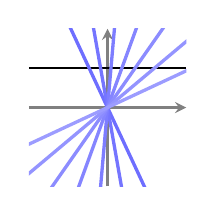
\begin{tikzpicture}
\draw[gray,thick,-stealth] (-1,0) -- (1,0);
\draw[gray,thick,-stealth] (0,-1) -- (0,1);
\draw[black,thick] (-1,.5) -- (1,.5);
\begin{scope}
    \clip(-1,-1) rectangle (1,1);
	\foreach \i in {1,...,7}
	{
		\pgfmathsetmacro\clr{100-5*\i}
		\pgfmathsetmacro\thet{130-15*\i}
		\draw[draw=curveOne!\clr,very thick] ({2*cos(\thet)},{2*sin(\thet)}) -- ({-2*cos(\thet)},{-2*sin(\thet)});
		\pgfmathsetmacro\xxx{cot(\thet)/2}
		\DrawDot{\xxx}{.5}
	}
\end{scope}
\DrawDot{0}{0}
\end{tikzpicture}
\end{document}
\end{center}
As we spin, our line strikes \(y=1\) at some point \((x,1)\), which we think of as a number \(x\); picture the line spinning clockwise, so \(x\to\infty\).
When our spinning line becomes horizontal, it becomes \(y=0\), so \(x=\infty\).
After that, as the angle of the line goes further around clockwise, we now find it strikes a point \((x,1)\) of our line \(y=1\) but with \(x<0\).
So we have ``passed through infinity'' and found ourselves wrapping around to negative numbers:
\begin{center}
\documentclass[tikz]{standalone}
\colorlet{curveZero}{gray!75}
\colorlet{curveOne}{blue!60}
\colorlet{curveTwo}{brown!50!gray}
\colorlet{curveThree}{green!40!gray}
\colorlet{curveFour}{red!50!gray}
\NewDocumentCommand\DrawDotInPlot{O{}mmO{}}%
{%
\fill[gray!20,draw=gray] (axis cs:{#2},{#3}) circle (1.3pt) node[above,black,#4] {\(#1\)};%
}%
\NewDocumentCommand\DrawDot{O{}mmO{}}%
{%
\fill[gray!20,draw=gray] ({#2},{#3}) circle (1.3pt) node[above,black,#4] {\(#1\)};%
}%
\NewDocumentCommand\DrawNode{O{}m}%
{%
\fill[gray!20,draw=gray] (#2) circle (1.3pt) node[above,black] {\(#1\)};%
}%
\colorlet{axisColor}{gray!50}
\tikzstyle{shapeZero}=[fill=curveZero,opacity=.4]
\tikzstyle{shapeOne}=[fill=curveOne,opacity=.4]
\tikzstyle{shapeTwo}=[fill=curveTwo,opacity=.4]
\tikzstyle{shapeThree}=[fill=curveThree,opacity=.4]
\tikzstyle{groupElementLabel}=[minimum size=2.4em]
\tikzstyle{groupElement}=[minimum size=2.4em,shapeZero,draw=curveZero]
\tikzstyle{cosetOne}=[minimum size=2.4em,shapeOne,draw=curveOne]
\tikzstyle{cosetTwo}=[minimum size=2.4em,shapeTwo,draw=curveTwo]


\begin{document}
\begin{tikzpicture}
\draw (0,0) circle (1cm);
\node[above] at (0,1) {\(0\)};
\node[below] at (0,-1) {\(\infty\)};
\node[left] at (-1,0) {\(-\)};
\node[right] at (1,0) {\(+\)};
\DrawDot{0}{1}
\DrawDot{0}{-1}
\end{tikzpicture}
\end{document}
\end{center}

The \emph{projective line}\define{projective line} of a field \(k\) is the set of all lines through the origin in the plane \(k^2\); each is uniquely expressed as \(x=ty\) for some element \(t\) from \(k\) (and so is naturally thought of as an element \(t\) of \(k\)), except for the line \(y=0\) (which we naturally write as \(t=\infty\)).
Every polynomial \(p(x)\), in one variable \(x\), of degree at most some positive integer \(d\), is naturally identified with a homogeneous polynomial \(P(x,y)\) of degree exactly \(d\), which then has roots in the projective line; to make sense of this, we must fix the choice of \(d\), some integer which is at least as large as the actual degree of \(p(x)\).
If \(p(x)\) has degree less than \(d\), say some degree \(d_0\), we can treat that as meaning that \(P(x,y)\) has \(d-d_0\) factors of \(y\), or say that \(p(x)\) has \(d-d_0\) ``roots at infinity''.
We are not afraid to work with roots at infinity, since we can always write out \(P(x,y)\) to make precise what we mean.
Roots won't disappear as we vary the coefficients of \(p(x)\), when we compute roots in the projective line; they only move to infinity, or even move across infinity.
We are forced to look for our roots on the projective line whenever we have a polynomial whose coefficients vary with some parameter.
\begin{problem}{projective.plane:lin.frac}
Suppose that we change variables \(x,y\) by a linear transformation, say to
\[
\begin{pmatrix}
X\\
Y
\end{pmatrix}
=
A
\begin{pmatrix}
x\\
y
\end{pmatrix}
\]
where
\[
A=
\begin{pmatrix}
a&b\\
c&d
\end{pmatrix}.
\]
Show that the line \(x=ty\) changes to the line \(X=TY\) given by the associated \emph{projective transformation}\define{projective transformation}
\[
T=\frac{at+b}{ct+d}.
\]
\end{problem}


\section{The projective plane}
\epigraph[author={Arthur Cayley}]{The more systematic course in the present introductory memoir \dots
would have been to ignore altogether the notions of distance and
metrical geometry \dots. Metrical geometry is a part of descriptive
geometry, and descriptive geometry is all geometry.}\SubIndex{Cayley, Arthur}%
The old fashioned term \emph{descriptive geometry}\define{descriptive geometry} means the geometry of straight lines.
Straight lines in the plane remain straight when you rescale the plane, or translate the plane to the left or right, up or down, or when you rotate the plane.
They even remain straight when you carry out any linear change of variables, as you know from linear algebra.

\bigskip

\epigraph[author={William Blake}, source={Auguries of Innocence}]{To see a World in a Grain of Sand, \\ And Heaven in a Wild Flower. \\ Hold Infinity in the palm of your hand, \\ And Eternity in an hour.}\SubIndex{Blake, William}%
Railway tracks built on a flat plane appear to meet ``at infinity''.
\begin{center}
\includegraphics[width=4cm]{railway-tracks.jpg} \\[2pt]
\begin{minipage}{4cm}\raggedright\tiny{Creative Commons Attribution-Share Alike 3.0 Unported license. I, MarcusObal}\end{minipage}
\end{center}
Imagine that we were to add a point to the plane ``at infinity'' in the direction where these tracks (straight lines) appear to meet.
\emph{Danger:} in order to add only one point, imagine that the two rails meet at the \emph{same} point in one direction as they do in the other, making them both into circles.
The projective plane is the set of all of the usual points of the plane (which we can think of as the ``finite points'' of the projective plane) together with some sort of ``points at infinity'' to represent the directions in the plane.

\epigraph[author={Fyodor Dostoyevsky}, source={The Brothers Karamazov}]{
But you must note this: if God exists and if He really did
create the world, then, as we all know, He created it according to
the geometry of Euclid and the human mind with the conception
of only three dimensions in space.  Yet there have been and
still are geometricians and philosophers, and even some of the
most distinguished, who doubt whether the whole universe, or
to speak more widely the whole of being, was only created in
Euclid's geometry; they even dare to dream that two parallel
lines, which according to Euclid can never meet on earth, may
meet somewhere in infinity.}\SubIndex{Dostoyevsky, Fyodor}\SubIndex{Brothers Karamazov}


We would like a more precise mathematical definition of points ``at infinity''.
Place yourself at a vantage point above the plane.
\begin{center}
\includegraphics[width=5cm]{above-the-plane-vantage}
\end{center}
Every ``finite'' point of the plane lies on a line through your vantage point: the line of sight.
\begin{center}
\includegraphics[width=5cm]{above-the-plane-connect}
\end{center}
You can also look out to the points at infinity, along lines:
\begin{center}
\includegraphics[width=5cm]{above-the-plane-off-to-infinity}
\end{center}
For example, there is such a line  parallel to the lines of our train track:
\begin{center}
\includegraphics[width=5cm]{above-the-plane-3}
\end{center}

On the other hand, if we take any line through the vantage point, either it hits a ``finite'' point of the plane:
\begin{center}
\includegraphics[width=5cm]{above-the-plane-connect}
\end{center}
or it is parallel to the plane
\begin{center}
\includegraphics[width=5cm]{above-the-plane-off-to-infinity}
\end{center}
so that it is pointed along the direction of some train tracks (lines) in the plane, to some ``point at infinity''.
\begin{center}
\includegraphics[width=5cm]{above-the-plane-3}
\end{center}
The points of the projective plane, finite points together with infinite points at infinity, are in 1-1 correspondence with lines through the vantage point.

This picture gives us a rigorous definition of points at infinity: the \emph{projective plane}\define{projective!plane} is the set of all lines through a chosen point of \(3\)-dimensional space, called the vantage point.
The \emph{points} of the projective plane (using this definition) are the lines through the vantage point.
The ``finite points'' are the lines not parallel to the horizontal plane, while the ``infinite points'' are the lines which are parallel the horizontal plane.
The set of finite points is the \emph{affine plane},\define{affine plane} which we think of as just the usual \(xy\)-plane.
The \emph{lines}\define{projective!line}, also called \emph{projective lines}, of the projective plane are the planes through the vantage point.
\begin{center}
\includegraphics[width=5cm]{above-the-plane-projective-line}
\end{center}

\section{Homogeneous coordinates}
We can make this more explicit by writing each point of \(3\)-dimensional space \(\R{3}\) as a triple \((x,y,z)\).
Draw the plane not as the usual \(xy\)-plane, but as the plane \(z=z_0\), for some nonzero constant \(z_0\).
Take the vantage point to be the origin.
Any linear change of the 3 variables \(x,y,z\) takes lines (and planes) through the origin to one another: there are more symmetries of the projective plane than we have ever encountered in the finite plane.

Every point of \(3\)-dimensional space not at the origin lies on a unique line through the origin.
So every point \((x,y,z)\) with not all of \(x,y,z\) zero lines on a unique line through the origin.
The points of this line are precisely the rescalings \((tx,ty,tz)\) of that point.
So each point of the projective plane can be written as a triple \((x,y,z)\), not all zero, and two such triples represent the same point just when each is a rescaling of the other.
Denote such a point as \([x,y,z]\).
For example, the point \([3,1,2]\) of the projective plane means the line through the origin consisting of the points of the form \((3t,t,2t)\) for all values of a variable \(t\), including \((3,1,2)\), \((3 \cdot 2, 1 \cdot 2, 2 \cdot 2)\), \((-3,-1,-2)\), and so on.
We write this as:
\[
[3,1,2]=[3 \cdot 2, 1 \cdot 2, 2 \cdot 2]=[-3,-1,-2].
\]
The coordinates \(x,y,z\) are the \emph{homogeneous coordinates}\define{homogeneous!coordinates}\define{coordinates!homogeneous} of a point \([x,y,z]\) of the projective plane.

In our pictures, the plane \(z=z_0\) was below the vantage point, but it is more traditional to take the plane to be \(z=1\), above the vantage point.
The \emph{affine plane} is just the usual \(xy\) plane, but identified either with the plane \(z=1\), or with the subset of the projective plane given by points \([x,y,1]\).

The roles of \(x,y,z\) are all the same now, and we can see that any linear change of variables of \(x,y,z\) takes the points of the projective plane to one another, and takes the lines of the projective plane to one another.
Each linear change of variables is represented by an invertible matrix
\[
g=
\begin{pmatrix}
g_{00} & g_{01} & g_{02} \\
g_{10} & g_{11} & g_{12} \\
g_{20} & g_{21} & g_{22}
\end{pmatrix}.
\]
Conventionally we label our matrix columns using \(0,1,2\) rather than \(1,2,3\).
Such a matrix takes a point \(p=[x,y,z]\) of the plane to the point \(q=[X,Y,Z]\) where
\[
\begin{pmatrix}
X \\
Y \\
Z
\end{pmatrix}
=
g
\begin{pmatrix}
x \\
y \\
z
\end{pmatrix}.
\]
We denote this relation as \(q=[g]p\) and call \([g]\) a \emph{projective automorphism}\define{projective!automorphism}.
Clearly if \(g\) and \(h\) are 2 invertible \(3 \times 3\) matrices, then \([gh]=[g][h]\), i.e. we carry out the transformation of lines through the origin by carrying out the multiplications by the matrices.

\begin{lemma}
If a square matrix \(g\) rescales every nonzero vector by a scalar, i.e. \(gx=\lambda(x)x\) for some number \(\lambda(x)\), for every vector \(x \ne 0\), then \(\lambda(x)\) is a constant scalar independent of \(x\), and \(g=\lambda I\) is a constant multiple of the identity matrix.
\end{lemma}
\begin{proof}
Suppose that \(g\) is \(n \times n\).
If \(n=1\) then every square matrix is a constant scalar, so suppose that \(n \ge 2\).
Write our vectors as \(x=\sum_j x_j e_j\) in the standard basis of \(\R{n}\) and calculate
\begin{align*}
gx
&=
\lambda\of{x} x,
\\
&=
\sum_j \lambda\of{x} x_j e_j,
\\
&=
\sum_j x_j ge_j,
\\
&=
\sum_j x_j \lambda\of{e_j} e_j.
\end{align*}
So for any \(x\) with \(x_j\ne 0\), we have \(\lambda(x)=\lambda\of{e_j}\).
But then if \(x_i \ne 0\), and if \(i \ne j\), then
\begin{align*}
\lambda(x) 
&=
\lambda\of{e_i},
\\
&=
\lambda\of{e_i+e_j},
\\
&=
\lambda\of{e_j}.
\end{align*}
So \(\lambda\) is a constant.
\end{proof}

\begin{lemma}
Two projective automorphisms \([g],[h]\) have precisely the same effect on all points \([x,y,z]\) of the projective plane just when the matrices agree up to a constant \(h=\lambda g\), some number \(\lambda \ne 0\).
\end{lemma}
\begin{proof}
Let \(\ell\defeq h^{-1}g\), so that \([\ell]=[h]^{-1}[g]\) and \([\ell]\) fixes every point of the projective plane just when \(\ell\) rescales every vector in \(\R{3}\) by  a scalar.
\end{proof} 

In particular, the points of the projective plane are permuted by the projective automorphisms, as are the projective lines.

The \emph{projective plane}\define{projective!plane} over any field \(k\), denoted \(\Proj[2]{k}\),\Notation{P2k}{\Proj[2]{k}}{projective plane over a field \(k\)} is the set of lines through the origin in \(k^3\).
In \(k^3\), the line through two points 
\[
p=
\begin{pmatrix}
x \\
y \\
z
\end{pmatrix},
q=
\begin{pmatrix}
X \\
Y \\
Z
\end{pmatrix}
\]
is just the set of all points \(tp+(1-t)q\) for \(t\) in \(k\).

\section{Example: the Fano plane}

Let \(k\defeq \Zmod{2}\); the \emph{Fano plane}\define{Fano plane}\define{plane!Fano} is the projective plane \(\Proj[2]{k}\).
Each point is \([x,y,z]\) with \(x,y,z\) in \(k\) defined up to rescaling.
But the only nonzero scalar you can use to rescale with is \(1\), since \(k=\Set{0,1}\).
Therefore we can just write \([x,y,z]\) as \((x,y,z)\).
Taking all possibilities for \(x,y,z\) from \(k\), not all zero, we get 7 points
\[
\begin{bmatrix}
1 \\
0 \\
0
\end{bmatrix},
\begin{bmatrix}
0 \\
1 \\
0
\end{bmatrix},
\begin{bmatrix}
1 \\
1 \\
0
\end{bmatrix},
\begin{bmatrix}
0 \\
0 \\
1
\end{bmatrix},
\begin{bmatrix}
1 \\
0 \\
1
\end{bmatrix},
\begin{bmatrix}
0 \\
1 \\
1
\end{bmatrix},
\begin{bmatrix}
1 \\
1 \\
1
\end{bmatrix},
\]
corresponding to the numbers \(1,2, \dots, 7\) written in base \(2\).

We can also draw this diagram as a cube; for each point, you draw the corresponding point in \(\R{3}\) with the same coordinates:
\begin{center}
\newcommand{\Depth}{1}
\newcommand{\Height}{1}
\newcommand{\Width}{1}
\tdplotsetmaincoords{70}{110}
\begin{tikzpicture}[tdplot_main_coords]
\coordinate (0) at (0,0,0);
\coordinate (1) at (\Depth,0,\Height);
\coordinate (2) at (\Depth,\Width,0);
\coordinate (3) at (0,\Width,\Height);
\coordinate (4) at (\Depth,\Width,\Height);
\coordinate (5) at (0,\Width,0);
\coordinate (6) at (0,0,\Height);
\coordinate (7) at (\Depth,0,0);

\draw[gray!10,fill=gray!10] (0) -- (6) -- (1) -- (7) -- cycle;% Left Face
\draw[gray!10,fill=gray!30] (0) -- (7) -- (2) -- (5) -- cycle;% Bottom Face
\draw[gray!10,fill=gray!40] (0) -- (6) -- (3) -- (5) -- cycle;% Back Face
\draw[gray!10,fill=gray!20,opacity=0.6] (1) -- (4) -- (2) -- (7) -- cycle;% Front Face
\draw[gray!10,fill=gray!20,opacity=0.8] (1) -- (4) -- (3) -- (6) -- cycle;% Top Face
\draw[gray!10,fill=gray!20,opacity=0.8] (4) -- (3) -- (5) -- (2) -- cycle;% Right Face

\node at (1) {\small\(6\)};
\node at (2) {\small\(3\)};
\node at (3) {\small\(5\)};
\node at (4) {\small\(7\)};
\node at (5) {\small\(1\)};
\node at (6) {\small\(4\)};
\node at (7) {\small\(2\)};

%% Following is for debugging purposes so you can see where the points are
%% These are last so that they show up on top
%\foreach \xy in {O, A, B, C, D, E, F, G}{
%    \node at (\xy) {\xy};
%}
\end{tikzpicture}
\end{center}
with one vertex not marked; the unmarked vertex is at the origin, so doesn't represent any point of the Fano plane.
Every line in the Fano plane has three vertices.
Take two numbers from 1 to 7, say \(1, 5\), and write out their binary digits under one another:
\[
\begin{array}{@{}c@{}c@{}c@{}}
0&0&1\\
1&0&1
\end{array}.
\]
Look at these as vectors in \(k^3\), so add them without carrying digits:
\[
\begin{array}{@{}c@{}c@{}c@{}}
0&0&1\\
1&0&1\\ \midrule
1&0&0
\end{array}
\]
The sum vector lies on the same line in the Fano plane, giving the lines:
\begin{center}
\newcommand{\Depth}{1}
\newcommand{\Height}{1}
\newcommand{\Width}{1}
\tdplotsetmaincoords{70}{110}
\begin{tikzpicture}[tdplot_main_coords]%Highlight the bottom
\coordinate (0) at (0,0,0);
\coordinate (1) at (\Depth,0,\Height);
\coordinate (2) at (\Depth,\Width,0);
\coordinate (3) at (0,\Width,\Height);
\coordinate (4) at (\Depth,\Width,\Height);
\coordinate (5) at (0,\Width,0);
\coordinate (6) at (0,0,\Height);
\coordinate (7) at (\Depth,0,0);
%

\draw[gray!10,fill=gray!10] (0) -- (6) -- (1) -- (7) -- cycle;% Left Face
\draw[gray!10,fill=gray!110] (0) -- (7) -- (2) -- (5) -- cycle;% Bottom Face
\draw[gray!10,fill=gray!40] (0) -- (6) -- (3) -- (5) -- cycle;% Back Face
\draw[gray!10,fill=gray!20,opacity=0.6] (1) -- (4) -- (2) -- (7) -- cycle;% Front Face
\draw[gray!10,fill=gray!20,opacity=0.8] (1) -- (4) -- (3) -- (6) -- cycle;% Top Face
\draw[gray!10,fill=gray!20,opacity=0.8] (4) -- (3) -- (5) -- (2) -- cycle;% Right Face

\node at (1) {\small\(6\)};
\node at (2) {\small\(3\)};
\node at (3) {\small\(5\)};
\node at (4) {\small\(7\)};
\node at (5) {\small\(1\)};
\node at (6) {\small\(4\)};
\node at (7) {\small\(2\)};

%% Following is for debugging purposes so you can see where the points are
%% These are last so that they show up on top
%\foreach \xy in {O, A, B, C, D, E, F, G}{
%    \node at (\xy) {\xy};
%}
\end{tikzpicture}
\begin{tikzpicture}[tdplot_main_coords]%Highlight the left
\coordinate (0) at (0,0,0);
\coordinate (1) at (\Depth,0,\Height);
\coordinate (2) at (\Depth,\Width,0);
\coordinate (3) at (0,\Width,\Height);
\coordinate (4) at (\Depth,\Width,\Height);
\coordinate (5) at (0,\Width,0);
\coordinate (6) at (0,0,\Height);
\coordinate (7) at (\Depth,0,0);
%

\draw[gray!10,fill=gray!90] (0) -- (6) -- (1) -- (7) -- cycle;% Left Face
\draw[gray!10,fill=gray!30] (0) -- (7) -- (2) -- (5) -- cycle;% Bottom Face
\draw[gray!10,fill=gray!40] (0) -- (6) -- (3) -- (5) -- cycle;% Back Face
\draw[gray!10,fill=gray!20,opacity=0.6] (1) -- (4) -- (2) -- (7) -- cycle;% Front Face
\draw[gray!10,fill=gray!20,opacity=0.8] (1) -- (4) -- (3) -- (6) -- cycle;% Top Face
\draw[gray!10,fill=gray!20,opacity=0.8] (4) -- (3) -- (5) -- (2) -- cycle;% Right Face

\node at (1) {\small\(6\)};
\node at (2) {\small\(3\)};
\node at (3) {\small\(5\)};
\node at (4) {\small\(7\)};
\node at (5) {\small\(1\)};
\node at (6) {\small\(4\)};
\node at (7) {\small\(2\)};

%% Following is for debugging purposes so you can see where the points are
%% These are last so that they show up on top
%\foreach \xy in {O, A, B, C, D, E, F, G}{
%    \node at (\xy) {\xy};
%}
\end{tikzpicture}
\begin{tikzpicture}[tdplot_main_coords]%Highlight back face
\coordinate (0) at (0,0,0);
\coordinate (1) at (\Depth,0,\Height);
\coordinate (2) at (\Depth,\Width,0);
\coordinate (3) at (0,\Width,\Height);
\coordinate (4) at (\Depth,\Width,\Height);
\coordinate (5) at (0,\Width,0);
\coordinate (6) at (0,0,\Height);
\coordinate (7) at (\Depth,0,0);
%

\draw[gray!10,fill=gray!10] (0) -- (6) -- (1) -- (7) -- cycle;% Left Face
\draw[gray!10,fill=gray!30] (0) -- (7) -- (2) -- (5) -- cycle;% Bottom Face
\draw[gray!10,fill=gray!120] (0) -- (6) -- (3) -- (5) -- cycle;% Back Face
\draw[gray!10,fill=gray!20,opacity=0.6] (1) -- (4) -- (2) -- (7) -- cycle;% Front Face
\draw[gray!10,fill=gray!20,opacity=0.8] (1) -- (4) -- (3) -- (6) -- cycle;% Top Face
\draw[gray!10,fill=gray!20,opacity=0.8] (4) -- (3) -- (5) -- (2) -- cycle;% Right Face

\node at (1) {\small\(6\)};
\node at (2) {\small\(3\)};
\node at (3) {\small\(5\)};
\node at (4) {\small\(7\)};
\node at (5) {\small\(1\)};
\node at (6) {\small\(4\)};
\node at (7) {\small\(2\)};

%% Following is for debugging purposes so you can see where the points are
%% These are last so that they show up on top
%\foreach \xy in {O, A, B, C, D, E, F, G}{
%    \node at (\xy) {\xy};
%}
\end{tikzpicture}
\begin{tikzpicture}[tdplot_main_coords]
\coordinate (0) at (0,0,0);
\coordinate (1) at (\Depth,0,\Height);
\coordinate (2) at (\Depth,\Width,0);
\coordinate (3) at (0,\Width,\Height);
\coordinate (4) at (\Depth,\Width,\Height);
\coordinate (5) at (0,\Width,0);
\coordinate (6) at (0,0,\Height);
\coordinate (7) at (\Depth,0,0);
%

\draw[gray!10,fill=gray!10] (0) -- (6) -- (1) -- (7) -- cycle;% Left Face
\draw[gray!10,fill=gray!30] (0) -- (7) -- (2) -- (5) -- cycle;% Bottom Face
\draw[gray!10,fill=gray!40] (0) -- (6) -- (3) -- (5) -- cycle;% Back Face
\draw[gray!10,fill=gray!20,opacity=0.6] (1) -- (4) -- (2) -- (7) -- cycle;% Front Face
\draw[gray!10,fill=gray!20,opacity=0.8] (1) -- (4) -- (3) -- (6) -- cycle;% Top Face
\draw[gray!10,fill=gray!20,opacity=0.8] (4) -- (3) -- (5) -- (2) -- cycle;% Right Face

\draw[gray!10,fill=gray!80,opacity=0.8] (0) -- (6) -- (4) -- (2) -- cycle;

\node at (1) {\small\(6\)};
\node at (2) {\small\(3\)};
\node at (3) {\small\(5\)};
\node at (4) {\small\(7\)};
\node at (5) {\small\(1\)};
\node at (6) {\small\(4\)};
\node at (7) {\small\(2\)};

%% Following is for debugging purposes so you can see where the points are
%% These are last so that they show up on top
%\foreach \xy in {O, A, B, C, D, E, F, G}{
%    \node at (\xy) {\xy};
%}
\end{tikzpicture}
\begin{tikzpicture}[tdplot_main_coords]
\coordinate (0) at (0,0,0);
\coordinate (1) at (\Depth,0,\Height);
\coordinate (2) at (\Depth,\Width,0);
\coordinate (3) at (0,\Width,\Height);
\coordinate (4) at (\Depth,\Width,\Height);
\coordinate (5) at (0,\Width,0);
\coordinate (6) at (0,0,\Height);
\coordinate (7) at (\Depth,0,0);
%

\draw[gray!10,fill=gray!10] (0) -- (6) -- (1) -- (7) -- cycle;% Left Face
\draw[gray!10,fill=gray!30] (0) -- (7) -- (2) -- (5) -- cycle;% Bottom Face
\draw[gray!10,fill=gray!40] (0) -- (6) -- (3) -- (5) -- cycle;% Back Face
\draw[gray!10,fill=gray!20,opacity=0.6] (1) -- (4) -- (2) -- (7) -- cycle;% Front Face
\draw[gray!10,fill=gray!20,opacity=0.8] (1) -- (4) -- (3) -- (6) -- cycle;% Top Face
\draw[gray!10,fill=gray!20,opacity=0.8] (4) -- (3) -- (5) -- (2) -- cycle;% Right Face

\draw[gray!10,fill=gray!80,opacity=0.8] (0) -- (1) -- (4) -- (5) -- cycle;

\node at (1) {\small\(6\)};
\node at (2) {\small\(3\)};
\node at (3) {\small\(5\)};
\node at (4) {\small\(7\)};
\node at (5) {\small\(1\)};
\node at (6) {\small\(4\)};
\node at (7) {\small\(2\)};

%% Following is for debugging purposes so you can see where the points are
%% These are last so that they show up on top
%\foreach \xy in {O, A, B, C, D, E, F, G}{
%    \node at (\xy) {\xy};
%}
\end{tikzpicture}
{
\tdplotsetmaincoords{50}{110}
\begin{tikzpicture}[tdplot_main_coords]
\coordinate (0) at (0,0,0);
\coordinate (1) at (\Depth,0,\Height);
\coordinate (2) at (\Depth,\Width,0);
\coordinate (3) at (0,\Width,\Height);
\coordinate (4) at (\Depth,\Width,\Height);
\coordinate (5) at (0,\Width,0);
\coordinate (6) at (0,0,\Height);
\coordinate (7) at (\Depth,0,0);

\draw[gray!10,fill=gray!10] (0) -- (6) -- (1) -- (7) -- cycle;% Left Face
\draw[gray!10,fill=gray!30] (0) -- (7) -- (2) -- (5) -- cycle;% Bottom Face
\draw[gray!10,fill=gray!40] (0) -- (6) -- (3) -- (5) -- cycle;% Back Face
\draw[gray!10,fill=gray!20,opacity=0.6] (1) -- (4) -- (2) -- (7) -- cycle;% Front Face
\draw[gray!10,fill=gray!20,opacity=0.8] (1) -- (4) -- (3) -- (6) -- cycle;% Top Face
\draw[gray!10,fill=gray!20,opacity=0.8] (4) -- (3) -- (5) -- (2) -- cycle;% Right Face

\draw[gray!10,fill=gray!80,opacity=0.8] (0) -- (7) -- (4) -- (3) -- cycle;

\node at (1) {\small\(6\)};
\node at (2) {\small\(3\)};
\node at (3) {\small\(5\)};
\node at (4) {\small\(7\)};
\node at (5) {\small\(1\)};
\node at (6) {\small\(4\)};
\node at (7) {\small\(2\)};

%% Following is for debugging purposes so you can see where the points are
%% These are last so that they show up on top
%\foreach \xy in {O, A, B, C, D, E, F, G}{
%    \node at (\xy) {\xy};
%}
\end{tikzpicture}
}
\begin{tikzpicture}[tdplot_main_coords]
\coordinate (0) at (0,0,0);
\coordinate (1) at (\Depth,0,\Height);
\coordinate (2) at (\Depth,\Width,0);
\coordinate (3) at (0,\Width,\Height);
\coordinate (4) at (\Depth,\Width,\Height);
\coordinate (5) at (0,\Width,0);
\coordinate (6) at (0,0,\Height);
\coordinate (7) at (\Depth,0,0);

\draw[gray!10,fill=gray!10] (0) -- (6) -- (1) -- (7) -- cycle;% Left Face
\draw[gray!10,fill=gray!30] (0) -- (7) -- (2) -- (5) -- cycle;% Bottom Face
\draw[gray!10,fill=gray!40] (0) -- (6) -- (3) -- (5) -- cycle;% Back Face
\draw[gray!10,fill=gray!20,opacity=0.6] (1) -- (4) -- (2) -- (7) -- cycle;% Front Face
\draw[gray!10,fill=gray!20,opacity=0.8] (1) -- (4) -- (3) -- (6) -- cycle;% Top Face
\draw[gray!10,fill=gray!20,opacity=0.8] (4) -- (3) -- (5) -- (2) -- cycle;% Right Face

\draw[gray!10,fill=gray!80,opacity=0.8] (1) -- (3) -- (2) -- cycle;

\node at (1) {\small\(6\)};
\node at (2) {\small\(3\)};
\node at (3) {\small\(5\)};
%\node at (4) {\small\(7\)};
\node at (5) {\small\(1\)};
\node at (6) {\small\(4\)};
\node at (7) {\small\(2\)};
\end{tikzpicture}
\end{center}


\section{Projective space}

Similarly, \emph{projective space}\define{projective!space} \(\Proj[n]{k}\)\Notation{Pnk}{\Proj[n]{k}}{projective space over a field \(k\)} is the set of lines through the origin of \(k^{n+1}\), and a \emph{projective automorphism}\define{projective!automorphism} of projective space is the result of applying an invertible square matrix to those lines.
Again, two invertible square matrices yield the same projective automorphism just when they agree up to a scalar multiple, by the same proof.
